\newcommand\PREAMBLE{}
\mode<article>
{
  \usepackage{fullpage}
  \usepackage{pgf}
  \usepackage{hyperref}
  \setjobnamebeamerversion{beamerexample2.beamer}
}

\mode<presentation>
{
%  \usetheme{Antibes}
%  \usetheme{Bergen}
%  \usetheme{Berkeley}
%  \usetheme{Berlin}
%  \usetheme{Boadilla} <-- OK
%  \usetheme{Copenhagen}
%  \usetheme{Darmstadt}
%  \usetheme{Dresden}
%  \usetheme{Frankfurt}
%  \usetheme{Goettingen}
%  \usetheme{Hannover}
%  \usetheme{Ilmenau}
%  \usetheme{JuanLesPins}
%  \usetheme{Madrid} <-- Good
%  \usetheme{Malmoe} <-- Good
%  \usetheme{Marburg}
%  \usetheme{Montpellier}
%  \usetheme{PaloAlto}
%  \usetheme{Pittsburgh}
%  \usetheme{Rochester} <-- Simple
  \usetheme{Singapore} %<-- Light, Good
%  \usetheme{Szeged}
%  \usetheme{academia}
  % or ...
%  \setbeamercovered{transparent}
  \setbeamercovered{invisible}
  \setbeamertemplate{navigation symbols}{} %remove navigation symbols
  % or whatever (possibly just delete it)
%  \universitylogo{ethlogo-black}
%  \departmentlogo{web_Icon}
}

\usepackage[english]{babel}
% or whatever

\usepackage[latin1]{inputenc}
% or whatever
\usepackage{times}
\usepackage[T1]{fontenc}

\usepackage{amsmath}
\usepackage{amssymb}
\usepackage[colour, nobox]{eventB}
\usepackage{bsymb}
\usepackage{spacing}
\usepackage{unitb}
\usepackage{unity}
\usepackage{ltl}
\usepackage[compact]{reqdoc}
\usepackage{reasoning}
\usepackage{tikz}
\usetikzlibrary{snakes,arrows}

%%%%% Some macros used in proof rules
%\newcommand{\Conv}[2]{\sequent{#1}{\downarrow #2}}
\newcommand{\Conv}[2]{\vdash \textsf{$#1$ is convergent in $#2$}}
%\newcommand{\Div}[2]{\sequent{#1}{\nearrow #2}}
\newcommand{\Div}[2]{\vdash \textsf{$#1$ is divergent in $#2$}}
%\newcommand{\DLF}[2]{\sequent{#1}{\circlearrowleft #2}}
\newcommand{\DLF}[2]{\vdash \textsf{$#1$ is deadlock-free in $#2$}}
%\newcommand{\LeadsFrom}[3]{\sequent{#1}{#2 \mathbin{\curvearrowright} #3}}
\newcommand{\LeadsFrom}[3]{\vdash \textsf{$#1$ leads from $#2$ to $#3$}}
\newcommand{\Pred}{P}
\newcommand{\Mch}{\Bmch{M}}

\title[The Unit-B Modelling Method]
 % (optional, use only with long paper titles)
{Progress Concerns as Design Guidelines}

%\subtitle

\author[S.~Hudon and T.S.~Hoang] % (optional, use only with lots of authors)
{Simon Hudon\inst{1} and Thai Son Hoang\inst{2}}

\institute[ETH-Z\"urich] %
%(optional, but mostly needed)
{
  \inst{1}Institute of Information Security, York University, Canada \\
  \inst{2}Institute of Information Security, ETH Zurich, Switzerland
}
% - Use the \inst command only if there are several affiliations.
% - Keep it simple, no one is interested in your street address.

\date[iFM 2013, 12/06/13]
% (optional, should be abbreviation of conference name)
{
  iFM 2013, Turku, Finland\\
  12th June 2013\\
}
% - Either use conference name or its abbreviation.
% - Not really informative to the audience, more for people (including
%   yourself) who are reading the slides online

\subject{Formal Methods}
% This is only inserted into the PDF information catalog. Can be left
% out. 


% Delete this, if you do not want the table of contents to pop up at
% the beginning of each section:
% \AtBeginSection[]
% {
%  \begin{frame}<beamer>
% % \begin{frame}
%    \frametitle{Outline}
%    \tableofcontents[currentsection]
%  \end{frame}
% }

\AtBeginSubsection[]
{
 \begin{frame}<beamer>
% \begin{frame}
   \frametitle{Outline}
   \tableofcontents[currentsection,currentsubsection]
 \end{frame}
}

% If you wish to uncover everything in a step-wise fashion, uncomment
% the following command:

%\beamerdefaultoverlayspecification{<+->}

\newcommand{\follows}{\Leftarrow}

\makeatletter
\newcommand*\dashV{\mathrel{\mathpalette\m@thr@fl@ct{\mathord\vDash}}}
\newcommand*\m@thr@fl@ct[2]{\reflectbox{$\m@th#1#2$}}
\makeatother
\newcommand{\abstracts}{\sqsubseteq}


\pgfdeclareimage[height=20ex]{out-of-order}{out-of-order}
\pgfdeclareimage[height=8ex]{ethz}{ethlogo-black}
\pgfdeclareimage[height=8ex]{yorku}{yorku}

\begin{document}


\logo{
  \vbox to \textheight{
    \vfil\hbox to 1.15\textwidth{
      \pgfuseimage{yorku}
      \hfil
      \pgfuseimage{ethz}
    }
  }
}
\begin{frame}
  \titlepage
\end{frame}
\logo{}

\begin{frame}
  \frametitle{Safety vs. Liveness}

  \begin{columns}
    \begin{column}{0.45\textwidth}
      \begin{block}{Liveness Properties}
        \begin{itemize}
        \item Something (good) \\
          \quad \alert{will happen}
          \medskip
        \item e.g. termination, progress
        \end{itemize}
      \end{block}
    \end{column}
    \begin{column}{0.45\textwidth}
      \begin{block}{Safety Properties}
        \begin{itemize}
        \item Something (bad) \\
          \quad \alert{never happens}.
          \medskip
        \item e.g. invariance properties
        \end{itemize}
      \end{block}
    \end{column}
  \end{columns}

  \vspace{2ex}

  \pause
  \begin{itemize}
  \item Liveness properties are \alert{desirable}.
    \pause
    
    \smallskip
    \begin{center}
      \pgfuseimage{out-of-order}
    \end{center}
    \pause
    \medskip
  \item Event-B does not support liveness properties.
  \end{itemize}

\end{frame}

\section{Formal Systems Development using Refinement}
\label{sec:form-syst-devel}

\begin{frame}
  \frametitle{Formal Systems Development using Refinement}

  \begin{itemize}
  \item To develop a system \Mch satisfying property $\phi$, i.e., $\Mch
    \models \phi$.
    \smallskip
    \begin{itemize}
    \item \Mch: some transition system
      \smallskip
    \item $\phi$: some logical formula
    \end{itemize}
    \medskip
  \item The main challenge: the \alert{complexity of the system}.
    \medskip
  \item \alert{Refinement} allows the step-by-step design of the
    system.
  \end{itemize}
\end{frame}

\begin{frame}
  \frametitle{Refinement}
  \framesubtitle{The UNITY way vs. the Event-B way}


  \begin{itemize}
  \item UNITY: Refines the \alert{formulae}.
    \[
    \lefteqn{\overbrace{\phantom{\phi \wide\follows \phi_1
          \wide\follows \ldots \wide\follows
          \phi_n}}^{\textsf{Refinement}}} \alert{\phi} \wide\follows \phi_1
    \wide\follows \ldots \wide\follows \underbrace{\phi_n \WIDE\dashV
      \alert{\Mch}}_{\textsf{Translation}}
    \]
    \begin{itemize}
    \item<2-> Cons: \alert{Hard to understand} the choice of refinement.
    \end{itemize}
    \medskip

  \item Event-B: Refines \alert{transition systems}.
    \[
    \lefteqn{
      \underbrace{\phantom{\phi \WIDE\dashV
        \Mch_0}}_{\textsf{Verification}}}  \alert{\phi} \WIDE\dashV
        \overbrace{\Mch_0 \wide\abstracts \Mch_1 \ldots \wide\abstracts \alert{\Mch}}^{\textsf{Refinement}}
    \]
    \begin{itemize}
    \item<2-> Cons: No support for \alert{liveness properties}.
    \end{itemize}
  \end{itemize}
\end{frame}

\begin{frame}
  \frametitle{The Unit-B Modelling Method}

  \begin{itemize}
  \item Inspired by UNITY and Event-B.
    \medskip
  \item Support the reasoning of \alert{liveness properties} (UNITY).
    \medskip
  \item \alert{Refinement} of transition systems (Event-B style).
    \medskip
  \item Developments using Unit-B are \\
    \alert{guided by both safety and liveness requirements}.
  \end{itemize}
\end{frame}


\begin{frame}
  \frametitle{Contributions}

  \begin{itemize}
  \item Event schedules: a generalisation of weakly and strongly fair
    assumptions.
    \medskip
  \item Refinement of event schedules preserving liveness properties.
  \end{itemize}
\end{frame}



\section{The Unit-B Modelling Method}
\label{sec:unit-b-modelling}
\begin{frame}<beamer>
  \frametitle{Outline}
  \tableofcontents[currentsection]
\end{frame}

\newBpar[pt]{t}
\newBvrb[vv]{v}
\newBcst{init}

\newcommand{\iI}{I}
\newcommand{\predP}{P}
\newcommand{\predQ}{Q}
\newcommand{\predR}{R}

\newBset[TRAIN]{TRN}
\newBvrb[trains]{trns}
\newBpar[train]{t}
\newBevt{arrive}
\newBevt{depart}
\newBinv[invTrainType]{inv0\_1}

\newBset[BLOCK]{BLK}
\newBcst{Entry}
\newBcst[PLATFORM]{PLF}
\newBcst{Exit}
\newBaxm[axmBlockType]{axm1\_1}
\newBvrb[location]{loc}
\newBinv[invLocationType]{inv1\_1}
\newBevt{moveout}
\newBevt{movein}

\newBset{COLOR}
\newBcst[GREEN]{GR}
\newBcst[RED]{RD}
\newBvrb[signal]{sgn}
\newBevt[ctrlplf]{ctrl\_platform}
\newBpar[platform]{p}

\begin{frame}
  \frametitle{Running Example. A Signal Control System}

  \begin{center}
    \ifx\PREAMBLE\UnDef
\documentclass{beamer}
\usepackage{tikz}
\usetikzlibrary{snakes,arrows}

\usepackage[english]{babel}
% or whatever

\usepackage[latin1]{inputenc}
% or whatever

\usepackage[T1]{fontenc}
\usepackage{amssymb}
\usepackage{amsmath}
\usepackage{eventB}

\begin{document}
\else
\fi


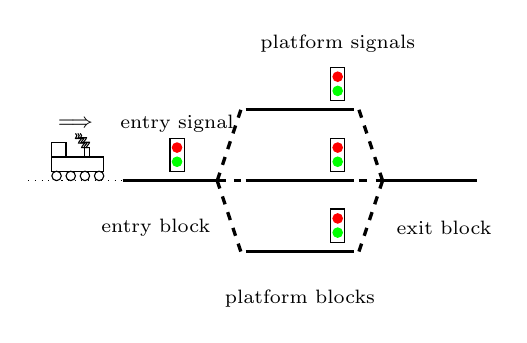
\begin{tikzpicture}[scale=0.6]
  \scriptsize
  % approaching block.
  \draw[very thick] (0,0) -- (1.5,0);
  \draw (0.7, -1) node{entry block};

  % in-switch
  \draw[very thick] (1.5,0) -- (2,0);
  \draw[very thick, dashed] (2,0) -- (2.5,1.5);
  \draw[very thick, dashed] (2,0) -- (2.5,-1.5);
  \draw[very thick, dashed] (2,0) -- (2.5,0);
%  \draw[red] (2, -1.5) node{in-switch};
  
  % platform blocks
  \draw[very thick] (2.6,0) -- (4.9,0);
%  \draw[very thick, dotted] (2.6,0.5) -- (4.9,0.5);
%  \draw[very thick, dotted] (2.6,-0.5) -- (4.9,-0.5);
  \draw[very thick] (2.6,1.5) -- (4.9,1.5);
  \draw[very thick] (2.6,-1.5) -- (4.9,-1.5);
  \draw (3.75, -2.5) node{platform blocks};

  % out-switch
  \draw[very thick] (5.5,0) -- (6,0);
  \draw[very thick, dashed] (5,1.5) -- (5.5,0);
  \draw[very thick, dashed] (5,0) -- (5.5,0);
  \draw[ very thick, dashed] (5,-1.5) -- (5.5,0);
%  \draw[red] (5.5, -1.5) node{out-switch};

  % exiting block.
  \draw[very thick] (6.0,0) -- (7.5,0);
  \draw (6.8, -1) node{exit block};

  % entry signal
%  \draw[very thick] (1.45,0) -- (1.45, 1);
  \draw (1, 0.2) rectangle +(0.3,0.7);
  \filldraw[red] (1.15, 0.7) circle (0.1);
  \filldraw[green] (1.15, 0.4) circle (0.1);
  \draw (1.15, 1.2) node{entry signal};

  % platform signals
%  \draw[very thick] (6.05,0) -- (6.05, 1);
  \draw (4.4, 0.2) rectangle +(0.3,0.7);
  \filldraw[red] (4.55, 0.7) circle (0.1);
  \filldraw[green] (4.55, 0.4) circle (0.1);
  \draw (4.55, 2.9) node{platform signals};

  \draw (4.4, 1.7) rectangle +(0.3,0.7);
  \filldraw[red] (4.55, 2.2) circle (0.1);
  \filldraw[green] (4.55, 1.9) circle (0.1);

  \draw (4.4, -1.3) rectangle +(0.3,0.7);
  \filldraw[red] (4.55, -0.8) circle (0.1);
  \filldraw[green] (4.55, -1.1) circle (0.1);

  % The train
  \draw[dotted] (-2,0) -- (0, 0);
  \draw(-1.5,0.2) rectangle +(1.1, 0.3);
  \draw(-1.5,0.5) rectangle +(0.3, 0.3);
  \draw(-0.8,0.5) rectangle +(0.1, 0.2);
  \draw[decorate, decoration={snake, amplitude = 1pt, segment length = 2pt}] (-0.8,0.7) --  (-1,1);
  \draw[decorate, decoration={snake, amplitude = 1pt, segment length = 2pt}] (-0.75,0.7) --  (-0.95,1);
  \draw[decorate, decoration={snake, amplitude = 1pt, segment length = 2pt}] (-0.7,0.7) --  (-0.9,1);
  \draw (-1.4, 0.1) circle (0.1);
  \draw (-1.1, 0.1) circle (0.1);
  \draw (-0.8, 0.1) circle (0.1);
  \draw (-0.5, 0.1) circle (0.1);
  \draw (-1, 1.2) node{$\Longrightarrow$};
\end{tikzpicture}

\ifx\PREAMBLE\UnDef
\end{document}
\else
\fi

  \end{center}
  
  \begin{requirements}
    \saf{saf:no-collision}{There is at most one train on each block}\ReqSpacing
    \live{live:train-leave}{Each train in the network eventually leaves}
  \end{requirements}
  
\end{frame}

\subsection{Unit-B Models}
\label{sec:unit-b-models}

\begin{frame}
  \frametitle{Unit-B Models -- Discrete Transition Systems}

  \begin{itemize}
  \item States are captured by \alert{variables $\vv$}.
    \medskip
  \item Transitions are modelled by \alert{guarded and scheduled events}.
  \end{itemize}

\end{frame}

\begin{frame}
  \frametitle{Traces and the Language of Temporal Logic}

  \begin{alertblock}{}
    A trace $\sigma$ is a (finite or infinite sequence of states)
    \[\sigma = s_0, s_1, s_2, s_3, \ldots\]
  \end{alertblock}

  \begin{itemize}
  \item A (basic) \structure{state formula} $\Pred$ is any
    \alert{first-order logic formula},
    \medskip
  \item The basic formulas can be extended by \structure{combining} \\
    \quad the \structure{Boolean operators} ($\neg, \land, \lor, \limp$) with
    \alert{temporal operators}:
    \medskip
    \begin{center}
      \ifx\PREAMBLE\UnDef
\documentclass{beamer}
\usepackage{tikz}
\usepackage[english]{babel}
% or whatever

\usepackage[latin1]{inputenc}
% or whatever
\usepackage{xifthen}
\usepackage{bsymb}

\newcommand{\always}{\mathop{\square}}
\newcommand{\eventually}{\mathop{\diamondsuit}}
\newcommand{\until}{\mathop{\mathcal{U}}}

\begin{document}
\else
\fi

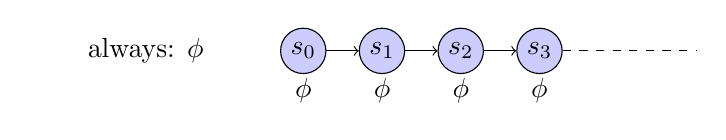
\begin{tikzpicture}[scale=0.5]
  \draw (-4,0) node[minimum width=3cm]{always: $\always \phi$};
  \draw (0,0) node(s0)[circle, draw, fill=blue!20!white, inner sep =
  2pt, minimum width=0.5cm]{$s_0$};
  \draw (2,0) node(s1)[circle, draw, fill=blue!20!white, inner sep =
  2pt, minimum width=0.5cm]{$s_1$};
  \draw (4,0) node(s2)[circle, draw, fill=blue!20!white, inner sep =
  2pt, minimum width=0.5cm]{$s_2$};
  \draw (6,0) node(s3)[circle, draw, fill=blue!20!white, inner sep =
  2pt, minimum width=0.5cm]{$s_3$};
  \draw[->] (s0) -- (s1);
  \draw[->] (s1) -- (s2);
  \draw[->] (s2) -- (s3);
  \draw[dashed] (s3) -- (10,0);
  \draw(0,-1) node{$\phi$};
  \draw(2,-1) node{$\phi$};
  \draw(4,-1) node{$\phi$};
  \draw(6,-1) node{$\phi$};
\end{tikzpicture}

\ifx\PREAMBLE\UnDef
\end{document}
\else
\fi

    \end{center}
    \begin{center}
      \ifx\PREAMBLE\UnDef
\documentclass{beamer}
\usepackage{tikz}
\usepackage[english]{babel}
% or whatever

\usepackage[latin1]{inputenc}
% or whatever
\usepackage{xifthen}
\usepackage{bsymb}

\newcommand{\always}{\mathop{\square}}
\newcommand{\eventually}{\mathop{\diamondsuit}}
\newcommand{\until}{\mathop{\mathcal{U}}}

\begin{document}
\else
\fi

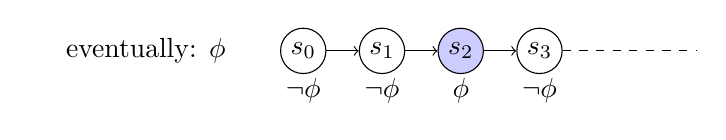
\begin{tikzpicture}[scale=0.5]
  \draw (-4,0) node[minimum width=3cm]{eventually: $\eventually \phi$};
  \draw (0,0) node(s0)[circle, draw, inner sep =
  2pt, minimum width=0.5cm]{$s_0$};
  \draw (2,0) node(s1)[circle, draw, inner sep =
  2pt, minimum width=0.5cm]{$s_1$};
  \draw (4,0) node(s2)[circle, draw, fill=blue!20!white, inner sep =
  2pt, minimum width=0.5cm]{$s_2$};
  \draw (6,0) node(s3)[circle, draw, inner sep =
  2pt, minimum width=0.5cm]{$s_3$};
  \draw[->] (s0) -- (s1);
  \draw[->] (s1) -- (s2);
  \draw[->] (s2) -- (s3);
  \draw[dashed] (s3) -- (10,0);
  \draw(0,-1) node{$\neg\phi$};
  \draw(2,-1) node{$\neg\phi$};
  \draw(4,-1) node{$\phi$};
  \draw(6,-1) node{$\neg\phi$};
\end{tikzpicture}

\ifx\PREAMBLE\UnDef
\end{document}
\else
\fi

    \end{center}
  \end{itemize}
\end{frame}

\begin{frame}
  \frametitle{Guarded events}

  \begin{columns}
    \begin{column}{0.3\textwidth}
      \[
      \ubevent{\evt}{\pt}{\guard.\pt.\vv}{}{}{\assignment.\pt.\vv.\vv'}
      \]
    \end{column}
    \begin{column}{0.5\textwidth}
      \begin{itemize}
      \item $\pt$: parameters
      \item $\guard.\pt.\vv$: guard
      \item $\assignment.\pt.\vv.\vv'$: action
      \end{itemize}
    \end{column}
  \end{columns}
  \medskip

  \begin{itemize}
  \item $\evt.\pt$ is \alert{enabled} when $\guard.\pt.\vv$ holds.
    \medskip
  \item Execution of $\evt.\pt$: \alert{$\vv$ is updated} according to the
    action $\assignment.\pt.\vv.\vv'$.
    \medskip
  \item $\evt.\pt$ corresponds to a formula $\act.(\evt.\pt)$.
  \end{itemize}
\end{frame}

\begin{frame}
  \frametitle{Scheduled events (1/2)}
  
  \begin{columns}
    \begin{column}{0.3\textwidth}
      \[
      \ubevent{\evt}{\pt}{\ldots}{
        \alert{\csched.\pt.\vv}
      }{
        \alert{\fsched.\pt.\vv}
      }
      {\ldots}
      \]
    \end{column}
    \begin{column}{0.5\textwidth}
      \begin{itemize}
      \item $\csched.\pt.\vv$: coarse-schedule.
        \medskip
      \item $\fsched.\pt.\vv$: fine-schedule.
        \medskip
      \item<2-> Healthiness condition: \[\csched.\pt.\vv \land
        \fsched.\pt.\vv \wide\limp \guard.\pt.\vv\]
      \end{itemize}
    \end{column}
  \end{columns}

  \medskip

  \begin{alertblock}{Liveness (Scheduling) Assumption}
    \begin{center}
      If $\csched.\pt.\vv$ holds infinitely long and $\fsched.\pt.\vv$
      holds infinitely often \\then eventually $\evt.\pt$ is executed.
      \[\schedule.(\evt.t) \Wide= \always (\always \csched \land \always \eventually \fsched
      \wide\limp \eventually (\act.(\evt.\pt)))\]
    \end{center}
  \end{alertblock}
\end{frame}

\begin{frame}
  \frametitle{Schedules vs. Fairness}
      \[
      \ubeventinline{\evt}{\pt}{\alert{\guard.\pt.\vv}}{
        \alert{\csched.\pt.\vv}
      }{
        \alert{\fsched.\pt.\vv}
      }
      {\ldots}
      \]

  \begin{itemize}
  \item Schedules are a \alert{generalisation} of weak- and
    strong-fairness.
    \medskip
  \item Weak-fairness:\\
    If \evt is \alert{enabled infinitely long} then \evt eventually occurs.
    \begin{itemize}
    \item Let $\csched$ be $\guard$ and $\fsched$ be $\btrue$.
    \end{itemize}
    \medskip
  \item Strong-fairness: \\
    If \evt is \alert{enabled infinitely often} then \evt eventually
    occurs.
    \begin{itemize}
    \item Let $\fsched$ be $\guard$ and $\csched$ be $\btrue$.
    \end{itemize}
  \end{itemize}
\end{frame}

\begin{frame}
  \frametitle{Scheduled events (2/2)}
  \framesubtitle{Conventions}

  \[
  \ubeventinline{\evt}{\pt}{\ldots}{
    \alert{\csched.\pt.\vv}
  }{
    \alert{\fsched.\pt.\vv}
  }
  {\ldots}
  \]
  
  \begin{itemize}
  \item \alert{Unscheduled} events (without \Bduring and \Bupon):
    \alert{$\csched$ is $\bfalse$}
    \medskip
  \item When only \Bduring is present (no \Bupon), \alert{$\fsched$ is $\btrue$}.
    \medskip
  \item When only \Bupon is present (no \Bduring), \alert{$\csched$ is
    $\btrue$}.
  \end{itemize}
\end{frame}


\begin{frame}
  \frametitle{Execution of Unit-B Models}

  \begin{align}
    \execution.\Mch \Wide{&=} \safety.\Mch \land
    \liveness.\Mch \\[2ex]
    \safety.\Mch  \Wide{&=}  \init \land \always \step.\Mch \\[2ex]
    \step.\Mch  \Wide{&=} (\exists \evt.t \in \Mch \qdot
    \act.(\evt.t)) \,\lor\, \SKIP \\[2ex]
    \liveness.\Mch \Wide{&=} \forall \evt.t \in \Mch \qdot
    \schedule.(\evt.t) \\[2ex]
    \schedule.(\evt.t) \WIDE{& =} \always (\always \csched
    \,\land\, \always \eventually \fsched  \wide{\limp} 
    \eventually (\fsched\land\act.(\evt.t)))
  \end{align}

\end{frame}

\begin{frame}
  \frametitle{A Signal Control System (Recall)}

  \begin{center}
    \ifx\PREAMBLE\UnDef
\documentclass{beamer}
\usepackage{tikz}
\usetikzlibrary{snakes,arrows}

\usepackage[english]{babel}
% or whatever

\usepackage[latin1]{inputenc}
% or whatever

\usepackage[T1]{fontenc}
\usepackage{amssymb}
\usepackage{amsmath}
\usepackage{eventB}

\begin{document}
\else
\fi


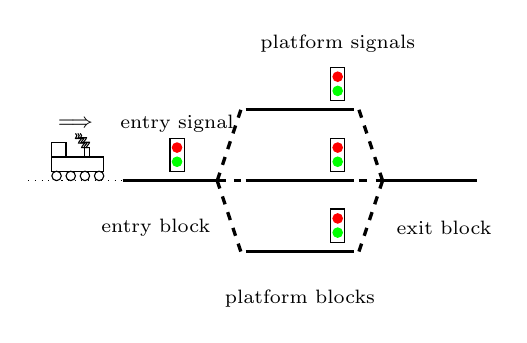
\begin{tikzpicture}[scale=0.6]
  \scriptsize
  % approaching block.
  \draw[very thick] (0,0) -- (1.5,0);
  \draw (0.7, -1) node{entry block};

  % in-switch
  \draw[very thick] (1.5,0) -- (2,0);
  \draw[very thick, dashed] (2,0) -- (2.5,1.5);
  \draw[very thick, dashed] (2,0) -- (2.5,-1.5);
  \draw[very thick, dashed] (2,0) -- (2.5,0);
%  \draw[red] (2, -1.5) node{in-switch};
  
  % platform blocks
  \draw[very thick] (2.6,0) -- (4.9,0);
%  \draw[very thick, dotted] (2.6,0.5) -- (4.9,0.5);
%  \draw[very thick, dotted] (2.6,-0.5) -- (4.9,-0.5);
  \draw[very thick] (2.6,1.5) -- (4.9,1.5);
  \draw[very thick] (2.6,-1.5) -- (4.9,-1.5);
  \draw (3.75, -2.5) node{platform blocks};

  % out-switch
  \draw[very thick] (5.5,0) -- (6,0);
  \draw[very thick, dashed] (5,1.5) -- (5.5,0);
  \draw[very thick, dashed] (5,0) -- (5.5,0);
  \draw[ very thick, dashed] (5,-1.5) -- (5.5,0);
%  \draw[red] (5.5, -1.5) node{out-switch};

  % exiting block.
  \draw[very thick] (6.0,0) -- (7.5,0);
  \draw (6.8, -1) node{exit block};

  % entry signal
%  \draw[very thick] (1.45,0) -- (1.45, 1);
  \draw (1, 0.2) rectangle +(0.3,0.7);
  \filldraw[red] (1.15, 0.7) circle (0.1);
  \filldraw[green] (1.15, 0.4) circle (0.1);
  \draw (1.15, 1.2) node{entry signal};

  % platform signals
%  \draw[very thick] (6.05,0) -- (6.05, 1);
  \draw (4.4, 0.2) rectangle +(0.3,0.7);
  \filldraw[red] (4.55, 0.7) circle (0.1);
  \filldraw[green] (4.55, 0.4) circle (0.1);
  \draw (4.55, 2.9) node{platform signals};

  \draw (4.4, 1.7) rectangle +(0.3,0.7);
  \filldraw[red] (4.55, 2.2) circle (0.1);
  \filldraw[green] (4.55, 1.9) circle (0.1);

  \draw (4.4, -1.3) rectangle +(0.3,0.7);
  \filldraw[red] (4.55, -0.8) circle (0.1);
  \filldraw[green] (4.55, -1.1) circle (0.1);

  % The train
  \draw[dotted] (-2,0) -- (0, 0);
  \draw(-1.5,0.2) rectangle +(1.1, 0.3);
  \draw(-1.5,0.5) rectangle +(0.3, 0.3);
  \draw(-0.8,0.5) rectangle +(0.1, 0.2);
  \draw[decorate, decoration={snake, amplitude = 1pt, segment length = 2pt}] (-0.8,0.7) --  (-1,1);
  \draw[decorate, decoration={snake, amplitude = 1pt, segment length = 2pt}] (-0.75,0.7) --  (-0.95,1);
  \draw[decorate, decoration={snake, amplitude = 1pt, segment length = 2pt}] (-0.7,0.7) --  (-0.9,1);
  \draw (-1.4, 0.1) circle (0.1);
  \draw (-1.1, 0.1) circle (0.1);
  \draw (-0.8, 0.1) circle (0.1);
  \draw (-0.5, 0.1) circle (0.1);
  \draw (-1, 1.2) node{$\Longrightarrow$};
\end{tikzpicture}

\ifx\PREAMBLE\UnDef
\end{document}
\else
\fi

  \end{center}
  
  \begin{description}
  \item[\ref{saf:no-collision}] {There is at most one train on each block}\ReqSpacing
  \item[\ref{live:train-leave}]{Each train in the network eventually leaves}
  \end{description}
  \medskip

  Refinement strategy: Prioritise ~\ref{live:train-leave} first.

\end{frame}


\begin{frame}
  \frametitle{A Signal Control System. The Initial Model}

  \begin{itemize}
  \item Focus on \alert{trains in the network}
    \medskip
  \item Set $\TRAIN$ denotes the set of possible trains.
    \medskip
  \item Variable \trains denotes the set of trains in the network.
    \medskip
  \item Event \arrive models a train entering the network.
    \medskip
  \item Event \depart models a train leaving the network.
  \end{itemize}
  \begin{Bcode}
    $
    \ubevent{\arrive}
    {\train}
    {\train \in \TRAIN}
    {}
    {}
    {\trains \bcmeq \trains \bunion \{\train\}}
    $
    \Bhspace
    $
    \ubevent{\depart}{\train}{\train \in \TRAIN}{\train \in \trains}{}{\trains \bcmeq \trains \setminus \{\train\}}
    $
  \end{Bcode}
\end{frame}


\subsection{Properties of Unit-B Models}
\label{sec:properties-unit-b}


\begin{frame}
  \frametitle{Execution and Properties}

  \begin{block}{Execution and Properties}
    \begin{center}
      \Mch satisfies $\phi$ \WIDE{if and only if} $\execution.\Mch \limp \phi$.
    \end{center}
  \end{block}

\end{frame}

\begin{frame}
  \frametitle{Safety Properties}

  \note{
    If $\predP$ holds at some point then
    \begin{itemize}
    \item $\predQ$ never  holds and $\predP$ continues to hold
      forever, or
      \smallskip
    \item $\predQ$ holds eventually and $\predP$ continues to hold
      at least until $\predQ$ holds.
    \end{itemize}
  }
  \begin{itemize}
  \item \alert{Invariance} properties: (in LTL $\always \iI$)
    \smallskip
    \begin{itemize}
    \item $\iI$ holds for every reachable state.
      \smallskip
    \item Proved using the standard \alert{induction technique}.
    \end{itemize}
    \medskip
  \item \alert{Unless} properties: $\predP \un \predQ$
    \smallskip
    \begin{itemize}
    \item if $\predP$ holds at some point then it continues to hold
      unless $\predQ$ holds.
      \smallskip
    \item Prove: If for every event
      \[
      \ubeventinline{\evt}{\pt}{\alert{\guard.\pt.\vv}}{
        \ldots
      }{
        \ldots
      }
      {\assignment.\pt.\vv.\vv'}
      \]
      in \Mch, we have
      \begin{equation}
        \predP.\vv \land \neg \predQ.\vv \land \guard.\pt.\vv \land \assignment.\pt.\vv.\vv'
        \WIDE\limp \predP.\vv' \lor \predQ.\vv'
        \tag{UN}
        \label{eq:UN}
      \end{equation}
      then \Mch satisfies $\predP \un \predQ$.
    \end{itemize}
  \end{itemize}

\end{frame}

\begin{frame}
  \frametitle{Liveness Properties}

  \begin{itemize}
  \item \alert{Progress} properties $\predP \leadsto
    \predQ$.
    \medskip
  \item In LTL: $\always (\predP \wide\limp \eventually \predQ)$
    \medskip
  \item Some important rules
  \begin{align}
    (\predP \limp \predQ) \WIDE{&\limp} (\predP \leadsto \predQ)
    \tag{Implication}\label{eq:implication} \\
    (\predP \leadsto \predQ) \land (\predQ \leadsto \predR) \WIDE{&\limp} (\predP \leadsto \predR)
    \tag{Transitivity}\label{eq:transitivity}
    \\
    \label{eq:37} 
    (\predP \leadsto \predQ)  \WIDE{&\leqv}  (\predP \,\land \! \neg \predQ \Wide{\leadsto} \predQ)
    \tag{Split-Off-Skip}
  \end{align}
  \end{itemize}
\end{frame}

\begin{frame}
  \frametitle{A Signal Control System. The Initial Model}
  \framesubtitle{Properties}
  \begin{description}
  \item[\ref{live:train-leave}]{Each train in the network eventually leaves}
  \end{description}
  \medskip
  \begin{Bcode}
    $
    \properties{
      \Binv{prg0\_1}: & \train \in \trains \wide\leadsto \train \notin
      \trains
    }
    $
  \end{Bcode}

  \medskip

  Note: Free-variables are universally quantified.
\end{frame}


\begin{frame}
  \frametitle{Transient Properties (1/3)}
  \framesubtitle{Definition}

  \begin{itemize}
  \item Borrowed from UNITY.
    \medskip
  \item The basic tool for reasoning about progress properties.
    \medskip
  \item $\tr \predP$ states that always \alert{$\predP$ is eventually
      falsified}.
    \medskip
  \item In LTL: $\always \eventually \neg \predP$. 
    \medskip
  \item Important properties:
    \[ \tr \predP \WIDE{=} \btrue \wide{\leadsto} \neg \predP  \WIDE{=} \predP \wide{\leadsto} \neg \predP 
 \]
  \end{itemize}
\end{frame}

\begin{frame}
  \frametitle{Transient Properties (2/3)}
  \begin{Theorem}[Implementing $\tr$]
    \label{thm:transient} if there exists an
    event
    \[\small
    \ubeventinline{\evt}{\pt}{\guard.\pt.\vv}{\csched.\pt.\vv}{\fsched.\pt.\vv}{\assignment.\pt.\vv.\vv'}
    \]
    in \Mch such that
    \begin{equation}
      \always (\predP \limp \csched)~,\label{eq:SCH}
      \tag{SCH}
    \end{equation}
    \begin{equation}
      \csched \leadsto \fsched~,\label{eq:OP}
      \tag{PRG}
    \end{equation}
    \begin{equation}
      \predP.\vv \land \csched.\pt.\vv \land \fsched.\pt.\vv \land \guard.\pt.\vv \land \assignment.\pt.\vv.\vv'
      \WIDE\limp \neg \predP.\vv'
      \tag{NEG}
      \label{eq:NEG}
    \end{equation}
    then  \Mch satisfies $\tr \predP$.
  \end{Theorem}

  \begin{itemize}
  \item \eqref{eq:SCH} corresponds to an invariance property.
    \smallskip
  \item \eqref{eq:OP} is trivial when $\fsched$ is $\btrue$.
    \smallskip
  \item \eqref{eq:NEG} corresponds to a standard Hoare-triple.
  \end{itemize}
\end{frame}

\begin{frame}
  \frametitle{Transient Properties (3/3)}
  \framesubtitle{A Sketch Proof}

  Consider $\tr \predP \Wide= \predP \leadsto \neg \predP \Wide= \always(\predP
  \limp \eventually \neg \predP)$. 

  \begin{proof}[Proof (Sketch)]
    Assume $\predP$ holds in some state, we prove $\eventually \neg
    \predP$ by contradiction.  \medskip
    \begin{enumerate}
    \item \label{asm} Assume \alert{$\always \predP$}.
      \medskip
    \item From \eqref{eq:SCH}, we have \alert{$\always \csched$},
      \medskip
    \item together with \eqref{eq:OP}, we have \alert{$\always \eventually
      \fsched$}.
      \medskip
    \item Scheduling assumption ensures that \alert{\evt will eventually
      occur}.
      \medskip
    \item \eqref{eq:NEG} guarantees that when \evt occurs, \alert{$\predP$ is
      falsified}.
    \medskip
    \item We have a \alert{contradiction} with the assumption from Step~\ref{asm}
    \end{enumerate}
  \end{proof}
\end{frame}

\begin{frame}
  \frametitle{A Signal Control System. The Initial Model}
  \framesubtitle{Properties}

  \note{%
    \Binv{prg0_1} holds no matter what the other events of the system
    are. In particular, we did not need to say that eventually, depart
    is the only event enabled. It is going to be executed because it
    is scheduled to. This is one strength of (weak) fairness.%
  }
  \begin{Bcode}[\small]
    $
    \ubevent{\depart}{\train}{\train \in \TRAIN}{\train \in
      \trains}{}{\trains \bcmeq \trains \setminus \{\train\}} $
    \Bhspace
    $ \properties[off]{ \Binv{prg0\_1}: & \train \in \trains
      \wide\leadsto \train \notin \trains } $
  \end{Bcode}

  \begin{itemize}
  \item $\Binv{prg0\_1}$ is the same as $\tr \train \in \trains$
    \medskip
  \item \eqref{eq:SCH} is trivial.
    \medskip
  \item No fine-schedule ($\fsched$ is $\btrue$) hence \eqref{eq:OP}
    is trivial.
    \medskip
  \item The event falsifies $\train \in \trains$ \eqref{eq:NEG}
  \end{itemize}
\end{frame}

\subsection{Refinement}
\label{sec:refinement}

\begin{frame}
  \frametitle{Refinement}

  \begin{itemize}
  \item Abstract systems can \alert{simulate} behaviours of concrete
    systems.
    \[\execution.\Bmch{cnc\Mch} \Wide\limp \execution.\Bmch{abs\Mch}\]
  \item \alert{Event-based} reasoning.
  \end{itemize}
  \medskip
  \begin{equation*}
    \ubeventinline{(abs\_)\evt}{\pt}{\guard}{\csched}{\fsched}{\assignment}\label{eq:absevt}
  \end{equation*}
  \begin{equation*}
    \ubeventinline{(cnc\_)\cncevt}{\pt}{\cncguard}{\cnccsched}{\cncfsched}{\cncassignment}\label{eq:cncevt}
  \end{equation*}
  
  \begin{itemize}
  \item Safety:
    \smallskip
    \begin{itemize}
    \item Guard strengthening: $\cncguard \limp \guard$
      \smallskip
    \item Action strengthening: $\cncassignment \limp \assignment$
    \end{itemize}
    \medskip
  \item Liveness:
    \smallskip
    \begin{itemize}
    \item Liveness assumption strengthening.
      \smallskip
    \item Schedules weakening: \[(\always \csched \wide\land \always
      \eventually \fsched) \WIDE\limp (\always \cnccsched \wide\land
      \always \eventually \cncfsched)\]
    \end{itemize}
  \end{itemize}
\end{frame}


\begin{frame}
  \frametitle{Schedules Weakening}
  \framesubtitle{Practical Rules}

  \note{
    This rule
    \begin{equation}
      \label{eq:fsched-strengthen}
      \cnccsched \land \cncfsched \wide\limp \fsched
    \end{equation}
  }
  
  \begin{equation}
    (\always \csched \wide\land \always
    \eventually \fsched) \WIDE\limp (\always \cnccsched \wide\land
    \always \eventually \cncfsched)\label{eq:ref-live}
    \tag{REF\_LIVE}
  \end{equation}
  \begin{itemize}
  \item<2-> \alert{Practical} rules:
    \medskip
    \begin{itemize}
    \item Coarse-schedule following
      \begin{equation}
        \label{eq:csched-weakening}
        \csched \land \fsched \wide\leadsto \cnccsched
        \tag{C\_FLW}
      \end{equation}
    \item Coarse-schedule stabilising
      \begin{equation}
        \label{eq:csched-stable}
        \cnccsched \wide\un \csched
        \tag{C\_STB}
      \end{equation}
    \item Fine-schedule following
      \begin{equation}
        \label{eq:fsched-weakening}
        \csched \land \fsched \wide\leadsto \cncfsched
        \tag{F\_FLW}
      \end{equation}
    \end{itemize}
  \end{itemize}
\end{frame}

% \begin{frame}
%   \frametitle{Schedules Weakening: Special Cases (1/4)}
%   \framesubtitle{Weakening the Coarse-Schedule}

%   \begin{equation*}
%     \ubeventinline{\evt}{\pt}{\ldots}{\csched}{\fsched}{\ldots}\label{eq:absevt}
%   \end{equation*}
%   \begin{equation*}
%     \ubeventinline{\cncevt}{\pt}{\ldots}{\cnccsched}{\fsched}{\ldots}\label{eq:cncevt}
%   \end{equation*}
  
%   \medskip

%   Conditions:

%   \begin{equation*}
%     \csched \wide\limp \cnccsched
%   \end{equation*}

% \end{frame}

% \begin{frame}
%   \frametitle{Schedules Weakening: Special Cases (3/4)}
%   \framesubtitle{Replacing the Coarse-schedule}

%   \begin{equation*}
%     \ubeventinline{\evt}{\pt}{\ldots}{\csched}{\fsched}{\ldots}\label{eq:absevt}
%   \end{equation*}
%   \begin{equation*}
%     \ubeventinline{\cncevt}{\pt}{\ldots}{\cnccsched}{\fsched}{\ldots}\label{eq:cncevt}
%   \end{equation*}

%   \medskip

%   Conditions:

%   \medskip

%   \begin{equation}
%     \csched \wide\leadsto \cnccsched
%     \tag{C\_WKN}
%   \end{equation}
%   \begin{equation}
%     \cnccsched \wide\un \csched
%     \tag{C\_STB}
%   \end{equation}

% \end{frame}

% \begin{frame}
%   \frametitle{Schedules Weakening: Special Cases (2/4)}
%   \framesubtitle{Strengthening the Coarse-schedule}

%   \begin{equation*}
%     \ubeventinline{\evt}{\pt}{\ldots}{\csched}{\fsched}{\ldots}\label{eq:absevt}
%   \end{equation*}
%   \begin{equation*}
%     \ubeventinline{\cncevt}{\pt}{\ldots}{\csched}{\fsched}{\ldots}\label{eq:cncevt}
%   \end{equation*}

% \end{frame}


\begin{frame}
  \frametitle{A Signal Control System. The First Refinement}
  \framesubtitle{The State}
  \begin{center}
    \ifx\PREAMBLE\UnDef
\documentclass{beamer}
\usepackage{tikz}
\usetikzlibrary{snakes,arrows}

\usepackage[english]{babel}
% or whatever

\usepackage[latin1]{inputenc}
% or whatever

\usepackage[T1]{fontenc}
\usepackage{amssymb}
\usepackage{amsmath}
\usepackage{eventB}

\begin{document}
\else
\fi


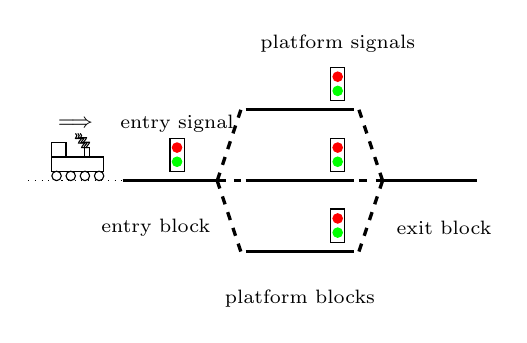
\begin{tikzpicture}[scale=0.6]
  \scriptsize
  % approaching block.
  \draw[very thick] (0,0) -- (1.5,0);
  \draw (0.7, -1) node{entry block};

  % in-switch
  \draw[very thick] (1.5,0) -- (2,0);
  \draw[very thick, dashed] (2,0) -- (2.5,1.5);
  \draw[very thick, dashed] (2,0) -- (2.5,-1.5);
  \draw[very thick, dashed] (2,0) -- (2.5,0);
%  \draw[red] (2, -1.5) node{in-switch};
  
  % platform blocks
  \draw[very thick] (2.6,0) -- (4.9,0);
%  \draw[very thick, dotted] (2.6,0.5) -- (4.9,0.5);
%  \draw[very thick, dotted] (2.6,-0.5) -- (4.9,-0.5);
  \draw[very thick] (2.6,1.5) -- (4.9,1.5);
  \draw[very thick] (2.6,-1.5) -- (4.9,-1.5);
  \draw (3.75, -2.5) node{platform blocks};

  % out-switch
  \draw[very thick] (5.5,0) -- (6,0);
  \draw[very thick, dashed] (5,1.5) -- (5.5,0);
  \draw[very thick, dashed] (5,0) -- (5.5,0);
  \draw[ very thick, dashed] (5,-1.5) -- (5.5,0);
%  \draw[red] (5.5, -1.5) node{out-switch};

  % exiting block.
  \draw[very thick] (6.0,0) -- (7.5,0);
  \draw (6.8, -1) node{exit block};

  % entry signal
%  \draw[very thick] (1.45,0) -- (1.45, 1);
  \draw (1, 0.2) rectangle +(0.3,0.7);
  \filldraw[red] (1.15, 0.7) circle (0.1);
  \filldraw[green] (1.15, 0.4) circle (0.1);
  \draw (1.15, 1.2) node{entry signal};

  % platform signals
%  \draw[very thick] (6.05,0) -- (6.05, 1);
  \draw (4.4, 0.2) rectangle +(0.3,0.7);
  \filldraw[red] (4.55, 0.7) circle (0.1);
  \filldraw[green] (4.55, 0.4) circle (0.1);
  \draw (4.55, 2.9) node{platform signals};

  \draw (4.4, 1.7) rectangle +(0.3,0.7);
  \filldraw[red] (4.55, 2.2) circle (0.1);
  \filldraw[green] (4.55, 1.9) circle (0.1);

  \draw (4.4, -1.3) rectangle +(0.3,0.7);
  \filldraw[red] (4.55, -0.8) circle (0.1);
  \filldraw[green] (4.55, -1.1) circle (0.1);

  % The train
  \draw[dotted] (-2,0) -- (0, 0);
  \draw(-1.5,0.2) rectangle +(1.1, 0.3);
  \draw(-1.5,0.5) rectangle +(0.3, 0.3);
  \draw(-0.8,0.5) rectangle +(0.1, 0.2);
  \draw[decorate, decoration={snake, amplitude = 1pt, segment length = 2pt}] (-0.8,0.7) --  (-1,1);
  \draw[decorate, decoration={snake, amplitude = 1pt, segment length = 2pt}] (-0.75,0.7) --  (-0.95,1);
  \draw[decorate, decoration={snake, amplitude = 1pt, segment length = 2pt}] (-0.7,0.7) --  (-0.9,1);
  \draw (-1.4, 0.1) circle (0.1);
  \draw (-1.1, 0.1) circle (0.1);
  \draw (-0.8, 0.1) circle (0.1);
  \draw (-0.5, 0.1) circle (0.1);
  \draw (-1, 1.2) node{$\Longrightarrow$};
\end{tikzpicture}

\ifx\PREAMBLE\UnDef
\end{document}
\else
\fi

  \end{center}
  \begin{itemize}
  \item Introduce the network topology: \BLOCK, \Entry, \PLATFORM, \Exit.
    \medskip
  \item Variable $\location$ denotes location of trains in the
    network.
    \medskip
    \begin{Bcode}
      $
      \invariants[off]{
        \Binv{inv1\_1}: \location \in \trains \tfun \BLOCK
      }
      $
    \end{Bcode}
  \end{itemize}
\end{frame}

\begin{frame}
  \frametitle{A Signal Control System. The First Refinement}
  \framesubtitle{Refinement of \depart}

  \begin{Bcode}
    $ \ubevent{(abs\_)\depart}{\train}{\train \in \TRAIN}{\train \in
      \trains}{}{\trains \bcmeq \trains \setminus \{\train\}} $
    \Bhspace
    $ \ubevent{(cnc\_)\depart}{\train}{ \train \in \trains \land
      \location.\train = \Exit } { \train \in \trains \land
      \location.\train = \Exit} {} {\trains \bcmeq \trains \setminus
      \{\train\} \\ \location \bcmeq \{\train\} \domsub \location} $
  \end{Bcode}

  \begin{itemize}
  \item Guard and action strengthening are trivial.
    \medskip
  \item Coarse-schedule following (amongst others):
    \begin{equation}
      \train \in \trains ~\leadsto~ \train \in \trains
      \land \location.\train = \Exit\label{eq:33}
      \tag{\Binv{prg1\_1}}
    \end{equation}
  \end{itemize}
\end{frame}

\begin{frame}
  \frametitle{A Signal Control System. The First Refinement}
  \framesubtitle{Refinement of \depart}
  
  \begin{Reason}
    \Step{}{
      \train \in \trains ~\leadsto~ \train \in \trains \land
      \location.\train = \Exit
    }
    \WideStepR{$\leqv$}{Put the negation of RHS in the LHS}{
      \train \in \trains \land \location.\train \neq \Exit ~\leadsto~ \train \in \trains \land
      \location.\train = \Exit
    }
    \WideStepR{$\follows$}{Transitivity}{
      \train \in \trains \land \location.\train \neq \Exit ~\leadsto~ \train \in \trains \land
      \location.\train \in \PLATFORM \Wide\land \\
      \train \in \trains \land \location.\train \in \PLATFORM ~\leadsto~ \train \in \trains \land
      \location.\train = \Exit
    }
  \end{Reason}

  \medskip

  \begin{itemize}
  \item The 1st condition is implemented by event \movein (not
    shown)
    \medskip

  \item The 2nd condition is implemented by event \moveout
    \medskip

  \item We need \alert{the ensure rule} (next slide).
  \end{itemize}

\end{frame}

\begin{frame}
  \frametitle{The Ensure Rule}
  
  \begin{Theorem}[The ensure-rule] For all state predicates $p$ and $q$,
    \label{thm:ensure-rule}
    \begin{equation}
      \label{eq:ensure-rule}
      \alert<4>{(\predP \un \predQ)} \wide\land \alert<2>{(\tr \, \predP \land \neg \predQ)}
      \WIDE\limp (\predP \leadsto \predQ)
      \tag{ENS}
    \end{equation}
    
    \begin{center}
      \ifx\PREAMBLE\UnDef
\documentclass{beamer}
\usepackage{tikz}
\usepackage[english]{babel}
% or whatever

\usepackage[latin1]{inputenc}
% or whatever
\usepackage{xifthen}
\usepackage{bsymb}
\usepackage{eventB}

\newcommand{\always}{\mathop{\square}}
\newcommand{\eventually}{\mathop{\diamondsuit}}
\newcommand{\until}{\mathop{\mathcal{U}}}
\newcommand{\predP}{P}
\newcommand{\predQ}{Q}

\begin{document}
\else
\fi

\begin{tikzpicture}[scale=1]
  \footnotesize
  \draw (0,0) node(s0)[circle, draw, inner sep =
  2pt, fill=blue!20!white, minimum width=0.7cm]{};
  \alt<1-2>{
    \draw (2,0) node(s1)[circle, draw, inner sep =
    2pt, fill=white!20!white, minimum width=0.7cm]{};
    \draw (4,0) node(s2)[circle, draw, inner sep =
    2pt, fill=white!20!white, minimum width=0.7cm]{};
  }
  {
    \draw (2,0) node(s1)[circle, draw, inner sep =
    2pt, fill=blue!20!white, minimum width=0.7cm]{};
    \draw (4,0) node(s2)[circle, draw, inner sep =
    2pt, fill=blue!20!white, minimum width=0.7cm]{};
  }
  \draw (6,0) node(s3)[circle, draw, inner sep =
  2pt, fill=red!20!white, minimum width=0.7cm]{};
  \draw[->,dashed] (-2,0) -- (s0);
  \draw[->] (s0) -- (s1);
  \draw[->] (s1) -- (s2);
  \draw[->] (s2) -- (s3);
  \draw[dashed] (s3) -- (8, 0);
  \draw (0,1) node{$\structure{\predP}$};
  \uncover<2->{\draw (6,-1) node{\alert<2,5>{$\neg \predP \lor \predQ$}};}
  \uncover<3->{
    \draw (4,-1.5) node{\alert<3>{$\predP \land \neg \predQ$}};
    \draw (2,-1.5) node{\alert<3>{$\predP \land \neg \predQ$}};
    \draw (0,-1.5) node{\alert<3>{$\predP \land \neg \predQ$}};
  }
  \uncover<4->{
    \draw (2, -2) node{\alert<4>{$\predP \lor \predQ$}};
    \draw (4, -2) node{\alert<4>{$\predP \lor \predQ$}};
    \draw (6, -2) node{\alert<4,5>{$\predP \lor \predQ$}};
  }
  % \uncover<4->{
  %   \draw (4,1) node{\structure{$\predP$}};
  %   \draw (2,1) node{\structure{$\predP$}};
  % }
  \uncover<5->{
    \draw (6, 1) node{\alert<5>{$\predQ$}};
  }
\end{tikzpicture}

\ifx\PREAMBLE\UnDef
\end{document}
\else
\fi

    \end{center}
  \end{Theorem}
\end{frame}

\begin{frame}
  \frametitle{A Signal Control System. The First Refinement}
  \framesubtitle{New Event \moveout}

  \begin{Reason}
    \Step{}{
      \train \in \trains \land \location.\train \in \PLATFORM ~\leadsto~ \train \in \trains \land
      \location.\train = \Exit
    }
    \WideStepR{$\follows$}{Ensure rule}{
      \train \in \trains \land \location.\train \in \PLATFORM ~\un~
      \train \in \trains \land \location.\train = \Exit \Wide\land \\
      (\tr \, (\train \in \trains \land \location.\train \in
      \PLATFORM) \land \neg(\train \in \trains \land \location.\train = \Exit))
    }
    \WideStepR{$\leqv$}{Logic}{
      \ldots \Wide\land (\tr \train \in \trains \land \location.\train \in \PLATFORM)
    }
  \end{Reason}
  
  \uncover<2->{
    \begin{Bcode}
      $
      \ubevent{\moveout}{\train}
      {\train \in \trains \land \location.\train \in \PLATFORM}
      {\train \in \trains \land \location.\train \in \PLATFORM}
      {}
      {\location.\train \bcmeq \Exit}
      $
    \end{Bcode}
  }
\end{frame}

\begin{frame}
  \frametitle{A Signal Control System. The Second Refinement}
  \framesubtitle{The State}
  
  \begin{description}
  \item[\ref{saf:no-collision}] {There is at most one train on each block}\ReqSpacing
  \end{description}
  \medskip
  \begin{Bcode}
    $
    \invariants[off]{
      \forall \train_1, \train_2 \Wide\qdot \train_1 \in \trains \land \train_2 \in \trains \land \location.\train_1 =
        \location.\train_2 \Wide\limp \train_1 = \train_2
    }
    $
  \end{Bcode}
\end{frame}

\begin{frame}
  \frametitle{A Signal Control System. The Second Refinement}
  \framesubtitle{Refinement of \moveout}
  \begin{Bcode}
      $
      \ubevent{(abs\_)\moveout}{\train}
      {\train \in \trains \land \location.\train \in \PLATFORM}
      {\train \in \trains \land \location.\train \in \PLATFORM}
      {}
      {\location.\train \bcmeq \Exit}
      $
      \Bhspace
    $ \ubevent{(cnc\_)\moveout}{\train}{ \train \in \trains \land
      \location.\train \in \PLATFORM \land \\
      \uncover<2->{\Exit \notin \ran.\location}}{\train \in \trains \land
      \location.\train \in \PLATFORM} {\uncover<3->{\Exit \notin \ran.\location}}
    {\location.\train \bcmeq \Exit} $
  \end{Bcode}

  \begin{itemize}
  \item<3-> Neither weak- nor strong-fairness is satisfactory.
    \smallskip
    \begin{itemize}
    \item Weak-fairness requires \Exit to be free infinitely long.
      \smallskip
    \item Strong-fairness is too strong assumption.
    \end{itemize}
  \end{itemize}
\end{frame}

\begin{frame}
  \frametitle{A Signal Control System. The Third Refinement}
  \framesubtitle{The State}

  \begin{itemize}
  \item Introduce the signals \signal

    \begin{Bcode}
      $ \invariants[false]{ \Binv{inv3\_1}: & \signal \in \{\Entry\}
        \bunion \PLATFORM \tfun
        \COLOR \\
        \Binv{inv3\_2}: & \forall p \qdot p \in \PLATFORM \land \signal.p =
          \GREEN \limp \Exit \notin \ran.\location \\
        \Binv{inv3\_3}: & \forall p,q \qdot p, q \in \PLATFORM \land
          \signal.p = \signal.q = \GREEN \limp p = q }$
    \end{Bcode}


  \end{itemize}

\end{frame}

\begin{frame}
  \frametitle{A Signal Control System. The Third Refinement}
  \framesubtitle{Refinement of \moveout}

  \begin{Bcode}[\footnotesize]
    $ \ubevent{(abs\_)\moveout}{\train}{ \train \in \trains \land
      \location.\train \in \PLATFORM \land \\
      \Exit \notin \ran.\location}{\train \in \trains \land
      \location.\train \in \PLATFORM} {\Exit \notin \ran.\location}
    {\location.\train \bcmeq \Exit} $
    \Bhspace
    $
    \ubevent{(cnc\_)\moveout}{\train}{
      \train \in \trains \land
      \location.\train \in \PLATFORM \land \\
      \signal.(\location.\train) = \GREEN
    }{\train \in \trains \land \location.train \in \PLATFORM \land \\
    \signal.(\location.\train) = \GREEN}{}{\location.\train \bcmeq
    \Exit \\
    \signal.(\location.\train) \bcmeq \RED
  }
  $
  \end{Bcode}

  \medskip
  Refinement requires to prove:
  \begin{equation}
    \label{eq:35}
    \tr \train \in \trains \land \location.\train \in
    \PLATFORM \land \signal.(\location.\train) = \RED~.
    \tag{\Binv{prg3\_5}}
  \end{equation}

\end{frame}

\begin{frame}
  \frametitle{A Signal Control System. The Third Refinement}
  \framesubtitle{New Controller Event \ctrlplf}

  \begin{Bcode}
    $
    \ubevent{\ctrlplf}{\platform}{
      \platform \in \PLATFORM \land
      \platform \in \ran.\location \land
      \Exit \notin \ran.\location \land \\
      (\forall q \qdot q \in \PLATFORM \limp \signal.q = \RED)
    }
    {
      \platform \in \PLATFORM \land
      \platform \in \ran.\location \land
      \signal.\platform = \RED
    }
    {
      \Exit \notin \ran(\location) \land
      (\forall q \qdot q \in \PLATFORM \land q \neq \platform \limp \signal.q = \RED)
    }
    {\signal.\platform \bcmeq \GREEN}
    $
  \end{Bcode}
\end{frame}

\section{Summary}
\label{sec:summary}

\begin{frame}
  \frametitle{Summary}
  \framesubtitle{The Unit-B Modelling Method}

  \begin{itemize}
  \item Guarded and \alert{scheduled} events.
    \medskip
  \item Reasoning about \alert{liveness (progress) properties}.
    \medskip
  \item \alert{Refinement} preserving safety and liveness properties.
    \medskip
  \item Developments are \alert{guided by safety and liveness requirements}.
  \end{itemize}
\end{frame}

\begin{frame}
  \frametitle{Summary}
  \framesubtitle{Future Work}

  \begin{itemize}
  \item Data refinement
    \medskip
  \item Decomposition / Composition
    \medskip
  \item Tool support
  \end{itemize}
\end{frame}

\begin{frame}[allowframebreaks]
  \frametitle{References}
  
  \begin{thebibliography}{10}
    
    % Start with overview books.
    \beamertemplatebookbibitems
  \bibitem[Hudon11]{hudon11:thesis}
    Simon Hudon.\\
    A Progress Preserving Refinement.\\
    \emph{Master Thesis}.\\
    Chair of Information Security, ETH Zurich, 2011.
    
    % Followed by interesting articles. Keep the list short. 
    \beamertemplatearticlebibitems
    
  \bibitem[HH13]{hh13:ifm}
    Simon Hudon and Thai Son Hoang.\\
    Systems Design Guided by Progress Concerns.\\
    Accepted for \emph{iFM 2013}.
    
  \end{thebibliography}
\end{frame}
\end{document}


%%% Local Variables: 
%%% mode: latex
%%% TeX-master: "unit-b-slides"
%%% End: 
